
%%%%%%%%%%%%%%%%%% PREAMBULE %%%%%%%%%%%%%%%%%%

\documentclass[aspectratio=169,utf8]{beamer}
%\documentclass[aspectratio=169,handout]{beamer}

\usetheme{Boadilla}
%\usecolortheme{seahorse}
\usecolortheme[RGB={245,66,24}]{structure}
\useoutertheme{infolines}

% packages
\usepackage{amsfonts,amsmath,amssymb,amsthm}
\usepackage[utf8]{inputenc}
\usepackage[T1]{fontenc}
\usepackage{lmodern}

\usepackage[francais]{babel}
\usepackage{fancybox}
\usepackage{graphicx}

\usepackage{float}
\usepackage{xfrac}

%\usepackage[usenames, x11names]{xcolor}
\usepackage{tikz}
\usepackage{pgfplots}
\usepackage{datetime}



%-----  Package unités -----
\usepackage{siunitx}
\sisetup{locale = FR,detect-all,per-mode = symbol}

%\usepackage{mathptmx}
%\usepackage{fouriernc}
%\usepackage{newcent}
%\usepackage[mathcal,mathbf]{euler}

%\usepackage{palatino}
%\usepackage{newcent}
% \usepackage[mathcal,mathbf]{euler}



% \usepackage{hyperref}
% \hypersetup{colorlinks=true, linkcolor=blue, urlcolor=blue,
% pdftitle={Exo7 - Exercices de mathématiques}, pdfauthor={Exo7}}


%section
% \usepackage{sectsty}
% \allsectionsfont{\bf}
%\sectionfont{\color{Tomato3}\upshape\selectfont}
%\subsectionfont{\color{Tomato4}\upshape\selectfont}

%----- Ensembles : entiers, reels, complexes -----
\newcommand{\Nn}{\mathbb{N}} \newcommand{\N}{\mathbb{N}}
\newcommand{\Zz}{\mathbb{Z}} \newcommand{\Z}{\mathbb{Z}}
\newcommand{\Qq}{\mathbb{Q}} \newcommand{\Q}{\mathbb{Q}}
\newcommand{\Rr}{\mathbb{R}} \newcommand{\R}{\mathbb{R}}
\newcommand{\Cc}{\mathbb{C}} 
\newcommand{\Kk}{\mathbb{K}} \newcommand{\K}{\mathbb{K}}

%----- Modifications de symboles -----
\renewcommand{\epsilon}{\varepsilon}
\renewcommand{\Re}{\mathop{\text{Re}}\nolimits}
\renewcommand{\Im}{\mathop{\text{Im}}\nolimits}
%\newcommand{\llbracket}{\left[\kern-0.15em\left[}
%\newcommand{\rrbracket}{\right]\kern-0.15em\right]}

\renewcommand{\ge}{\geqslant}
\renewcommand{\geq}{\geqslant}
\renewcommand{\le}{\leqslant}
\renewcommand{\leq}{\leqslant}
\renewcommand{\epsilon}{\varepsilon}

%----- Fonctions usuelles -----
\newcommand{\ch}{\mathop{\text{ch}}\nolimits}
\newcommand{\sh}{\mathop{\text{sh}}\nolimits}
\renewcommand{\tanh}{\mathop{\text{th}}\nolimits}
\newcommand{\cotan}{\mathop{\text{cotan}}\nolimits}
\newcommand{\Arcsin}{\mathop{\text{arcsin}}\nolimits}
\newcommand{\Arccos}{\mathop{\text{arccos}}\nolimits}
\newcommand{\Arctan}{\mathop{\text{arctan}}\nolimits}
\newcommand{\Argsh}{\mathop{\text{argsh}}\nolimits}
\newcommand{\Argch}{\mathop{\text{argch}}\nolimits}
\newcommand{\Argth}{\mathop{\text{argth}}\nolimits}
\newcommand{\pgcd}{\mathop{\text{pgcd}}\nolimits} 


%----- Commandes divers ------
\newcommand{\ii}{\mathrm{i}}
\newcommand{\dd}{\text{d}}
\newcommand{\id}{\mathop{\text{id}}\nolimits}
\newcommand{\Ker}{\mathop{\text{Ker}}\nolimits}
\newcommand{\Card}{\mathop{\text{Card}}\nolimits}
\newcommand{\Vect}{\mathop{\text{Vect}}\nolimits}
\newcommand{\Mat}{\mathop{\text{Mat}}\nolimits}
\newcommand{\rg}{\mathop{\text{rg}}\nolimits}
\newcommand{\tr}{\mathop{\text{tr}}\nolimits}


%----- Structure des exercices ------

\newtheoremstyle{styleexo}% name
{2ex}% Space above
{3ex}% Space below
{}% Body font
{}% Indent amount 1
{\bfseries} % Theorem head font
{}% Punctuation after theorem head
{\newline}% Space after theorem head 2
{}% Theorem head spec (can be left empty, meaning ‘normal’)

%\theoremstyle{styleexo}
\newtheorem{exo}{Exercice}
\newtheorem{ind}{Indications}
\newtheorem{cor}{Correction}


\newcommand{\exercice}[1]{} \newcommand{\finexercice}{}
%\newcommand{\exercice}[1]{{\tiny\texttt{#1}}\vspace{-2ex}} % pour afficher le numero absolu, l'auteur...
\newcommand{\enonce}{\begin{exo}} \newcommand{\finenonce}{\end{exo}}
\newcommand{\indication}{\begin{ind}} \newcommand{\finindication}{\end{ind}}
\newcommand{\correction}{\begin{cor}} \newcommand{\fincorrection}{\end{cor}}

\newcommand{\noindication}{\stepcounter{ind}}
\newcommand{\nocorrection}{\stepcounter{cor}}

\newcommand{\fiche}[1]{} \newcommand{\finfiche}{}
\newcommand{\titre}[1]{\centerline{\large \bf #1}}
\newcommand{\addcommand}[1]{}
\newcommand{\video}[1]{}

% Marge
\newcommand{\mymargin}[1]{\marginpar{{\small #1}}}

\def\noqed{\renewcommand{\qedsymbol}{}}


%----- Presentation ------
\setlength{\parindent}{0cm}

%\newcommand{\ExoSept}{\href{http://exo7.emath.fr}{\textbf{\textsf{Exo7}}}}

\definecolor{myred}{rgb}{0.93,0.26,0}
\definecolor{myorange}{rgb}{0.97,0.58,0}
\definecolor{myyellow}{rgb}{1,0.86,0}

\newcommand{\LogoExoSept}[1]{  % input : echelle
{\usefont{U}{cmss}{bx}{n}
\begin{tikzpicture}[scale=0.1*#1,transform shape]
  \fill[color=myorange] (0,0)--(4,0)--(4,-4)--(0,-4)--cycle;
  \fill[color=myred] (0,0)--(0,3)--(-3,3)--(-3,0)--cycle;
  \fill[color=myyellow] (4,0)--(7,4)--(3,7)--(0,3)--cycle;
  \node[scale=5] at (3.5,3.5) {Exo7};
\end{tikzpicture}}
}


\newcommand{\debutmontitre}{
  \author{} \date{} 
  \thispagestyle{empty}
  \hspace*{-10ex}
  \begin{minipage}{\textwidth}
    \titlepage  
  \vspace*{-2.5cm}
  \begin{center}
    \LogoExoSept{2.5}
  \end{center}
  \end{minipage}

  \vspace*{-0cm}
  
  % Astuce pour que le background ne soit pas discrétisé lors de la conversion pdf -> png
\begin{tikzpicture}
        \fill[opacity=0,green!60!black] (0,0)--++(0,0)--++(0,0)--++(0,0)--cycle; 
\end{tikzpicture}

% toc S'affiche trop tot :
% \tableofcontents[hideallsubsections, pausesections]
}

\newcommand{\finmontitre}{
  \end{frame}
  \setcounter{framenumber}{0}
} % ne marche pas pour une raison obscure

%----- Commandes supplementaires ------

% \usepackage[landscape]{geometry}
% \geometry{top=1cm, bottom=3cm, left=2cm, right=10cm, marginparsep=1cm
% }
% \usepackage[a4paper]{geometry}
% \geometry{top=2cm, bottom=2cm, left=2cm, right=2cm, marginparsep=1cm
% }

%\usepackage{standalone}


% New command Arnaud -- november 2011
\setbeamersize{text margin left=24ex}
% si vous modifier cette valeur il faut aussi
% modifier le decalage du titre pour compenser
% (ex : ici =+10ex, titre =-5ex

\theoremstyle{definition}
%\newtheorem{proposition}{Proposition}
%\newtheorem{exemple}{Exemple}
%\newtheorem{theoreme}{Théorème}
%\newtheorem{lemme}{Lemme}
%\newtheorem{corollaire}{Corollaire}
%\newtheorem*{remarque*}{Remarque}
%\newtheorem*{miniexercice}{Mini-exercices}
%\newtheorem{definition}{Définition}

% Commande tikz
\usetikzlibrary{calc}
\usetikzlibrary{patterns,arrows}
\usetikzlibrary{matrix}
\usetikzlibrary{fadings} 

%definition d'un terme
\newcommand{\defi}[1]{{\color{myorange}\textbf{\emph{#1}}}}
\newcommand{\evidence}[1]{{\color{blue}\textbf{\emph{#1}}}}
\newcommand{\assertion}[1]{\emph{\og#1\fg}}  % pour chapitre logique
%\renewcommand{\contentsname}{Sommaire}
\renewcommand{\contentsname}{}
\setcounter{tocdepth}{2}



%------ Figures ------

\def\myscale{1} % par défaut 
\newcommand{\myfigure}[2]{  % entrée : echelle, fichier figure
\def\myscale{#1}
\begin{center}
\footnotesize
{#2}
\end{center}}


%------ Encadrement ------

\usepackage{fancybox}


\newcommand{\mybox}[1]{
\setlength{\fboxsep}{7pt}
\begin{center}
\shadowbox{#1}
\end{center}}

\newcommand{\myboxinline}[1]{
\setlength{\fboxsep}{5pt}
\raisebox{-10pt}{
\shadowbox{#1}
}
}

%--------------- Commande beamer---------------
\newcommand{\beameronly}[1]{#1} % permet de mettre des pause dans beamer pas dans poly


\setbeamertemplate{navigation symbols}{}
\setbeamertemplate{footline}  % tiré du fichier beamerouterinfolines.sty
{
  \leavevmode%
  \hbox{%
  \begin{beamercolorbox}[wd=.333333\paperwidth,ht=2.25ex,dp=1ex,center]{author in head/foot}%
    % \usebeamerfont{author in head/foot}\insertshortauthor%~~(\insertshortinstitute)
    \usebeamerfont{section in head/foot}{\bf\insertshorttitle}
  \end{beamercolorbox}%
  \begin{beamercolorbox}[wd=.333333\paperwidth,ht=2.25ex,dp=1ex,center]{title in head/foot}%
    \usebeamerfont{section in head/foot}{\bf\insertsectionhead}
  \end{beamercolorbox}%
  \begin{beamercolorbox}[wd=.333333\paperwidth,ht=2.25ex,dp=1ex,right]{date in head/foot}%
    % \usebeamerfont{date in head/foot}\insertshortdate{}\hspace*{2em}
    \insertframenumber{} / \inserttotalframenumber\hspace*{2ex} 
  \end{beamercolorbox}}%
  \vskip0pt%
}


\definecolor{mygrey}{rgb}{0.5,0.5,0.5}
\setlength{\parindent}{0cm}
%\DeclareTextFontCommand{\helvetica}{\fontfamily{phv}\selectfont}

% background beamer
\definecolor{couleurhaut}{rgb}{0.85,0.9,1}  % creme
\definecolor{couleurmilieu}{rgb}{1,1,1}  % vert pale
\definecolor{couleurbas}{rgb}{0.85,0.9,1}  % blanc
\setbeamertemplate{background canvas}[vertical shading]%
[top=couleurhaut,middle=couleurmilieu,midpoint=0.4,bottom=couleurbas] 
%[top=fondtitre!05,bottom=fondtitre!60]



\makeatletter
\setbeamertemplate{theorem begin}
{%
  \begin{\inserttheoremblockenv}
  {%
    \inserttheoremheadfont
    \inserttheoremname
    \inserttheoremnumber
    \ifx\inserttheoremaddition\@empty\else\ (\inserttheoremaddition)\fi%
    \inserttheorempunctuation
  }%
}
\setbeamertemplate{theorem end}{\end{\inserttheoremblockenv}}

\newenvironment{theoreme}[1][]{%
   \setbeamercolor{block title}{fg=structure,bg=structure!40}
   \setbeamercolor{block body}{fg=black,bg=structure!10}
   \begin{block}{{\bf Th\'eor\`eme }#1}
}{%
   \end{block}%
}


\newenvironment{proposition}[1][]{%
   \setbeamercolor{block title}{fg=structure,bg=structure!40}
   \setbeamercolor{block body}{fg=black,bg=structure!10}
   \begin{block}{{\bf Proposition }#1}
}{%
   \end{block}%
}

\newenvironment{corollaire}[1][]{%
   \setbeamercolor{block title}{fg=structure,bg=structure!40}
   \setbeamercolor{block body}{fg=black,bg=structure!10}
   \begin{block}{{\bf Corollaire }#1}
}{%
   \end{block}%
}

\newenvironment{mydefinition}[1][]{%
   \setbeamercolor{block title}{fg=structure,bg=structure!40}
   \setbeamercolor{block body}{fg=black,bg=structure!10}
   \begin{block}{{\bf Définition} #1}
}{%
   \end{block}%
}

\newenvironment{lemme}[0]{%
   \setbeamercolor{block title}{fg=structure,bg=structure!40}
   \setbeamercolor{block body}{fg=black,bg=structure!10}
   \begin{block}{\bf Lemme}
}{%
   \end{block}%
}

\newenvironment{remarque}[1][]{%
   \setbeamercolor{block title}{fg=black,bg=structure!20}
   \setbeamercolor{block body}{fg=black,bg=structure!5}
   \begin{block}{Remarque #1}
}{%
   \end{block}%
}


\newenvironment{exemple}[1][]{%
   \setbeamercolor{block title}{fg=black,bg=structure!20}
   \setbeamercolor{block body}{fg=black,bg=structure!5}
   \begin{block}{{\bf Exemple }#1}
}{%
   \end{block}%
}


\newenvironment{miniexercice}[0]{%
   \setbeamercolor{block title}{fg=structure,bg=structure!20}
   \setbeamercolor{block body}{fg=black,bg=structure!5}
   \begin{block}{Mini-exercices}
}{%
   \end{block}%
}


\newenvironment{tp}[0]{%
   \setbeamercolor{block title}{fg=structure,bg=structure!40}
   \setbeamercolor{block body}{fg=black,bg=structure!10}
   \begin{block}{\bf Travaux pratiques}
}{%
   \end{block}%
}
\newenvironment{exercicecours}[1][]{%
   \setbeamercolor{block title}{fg=structure,bg=structure!40}
   \setbeamercolor{block body}{fg=black,bg=structure!10}
   \begin{block}{{\bf Exercice }#1}
}{%
   \end{block}%
}
\newenvironment{algo}[1][]{%
   \setbeamercolor{block title}{fg=structure,bg=structure!40}
   \setbeamercolor{block body}{fg=black,bg=structure!10}
   \begin{block}{{\bf Algorithme}\hfill{\color{gray}\texttt{#1}}}
}{%
   \end{block}%
}


\setbeamertemplate{proof begin}{
   \setbeamercolor{block title}{fg=black,bg=structure!20}
   \setbeamercolor{block body}{fg=black,bg=structure!5}
   \begin{block}{{\footnotesize Démonstration}}
   \footnotesize
   \smallskip}
\setbeamertemplate{proof end}{%
   \end{block}}
\setbeamertemplate{qed symbol}{\openbox}


\makeatother
\usecolortheme[RGB={192,41,0}]{structure}

% Commande spécifique à ce chapitre
\newcommand{\Sage}{\texttt{Sage}}

\usepackage{textcomp}

\usepackage{listings}
\lstset{
  upquote=true,
  columns=flexible,
  keepspaces=true,
  basicstyle=\ttfamily,
  commentstyle=\color{gray},
  language=Python,
  showstringspaces=false,
  aboveskip=0em,  
  belowskip=0em,
  escapeinside=||,
  breaklines=true,
  postbreak=\raisebox{0ex}[0ex][0ex]{\qquad\ensuremath{\color{red}\hookrightarrow\space}},
}

\lstset{
  literate={é}{{\'e}}1
           {è}{{\`e}}1
           {à}{{\`a}}1
}

\newcommand{\codeinline}[1]{\lstinline!#1!}

  
%%%%%%%%%%%%%%%%%%%%%%%%%%%%%%%%%%%%%%%%%%%%%%%%%%%%%%%%%%%%%
%%%%%%%%%%%%%%%%%%%%%%%%%%%%%%%%%%%%%%%%%%%%%%%%%%%%%%%%%%%%%


\begin{document}

\renewcommand*{\theenumii}{\alph{enumii}}

\title{{\bf Calcul formel}}
\subtitle{Polynômes}

\begin{frame}
  
  \debutmontitre

  \pause

{\footnotesize
\hfill
\setbeamercovered{transparent=50}
\begin{minipage}{0.6\textwidth}
  \begin{itemize}
    \item<3-> Manipuler les polynômes
    \item<4-> Algorithme de Horner
    \item<5-> Interpolation de Lagrange
  \end{itemize}
\end{minipage}
}

\end{frame}

\setcounter{framenumber}{0}





%%%%%%%%%%%%%%%%%%%%%%%%%%%%%%%%%%%%%%%%%%%%%%%%%%%%%%%%%%%%%%%%
\section{Manipuler les polynômes}

\begin{frame}[fragile]
\begin{tp}
Soient  $P(X) = X^4-3X^2-1$ et $Q(X) = (X+1)^4$ des polynômes de $\Qq[X]$.
Après avoir déclaré l'anneau des polynômes $\Qq[X]$ par \codeinline{R.<X> = QQ[]} 
(où \codeinline{QQ} désigne le corps des rationnels), répondre aux questions suivantes : \pause
\begin{enumerate}
  \item Est-ce que $\deg(P \cdot Q) = \deg P + \deg Q$ ?\pause
  \item Est-ce que $\deg(P - Q) = \max( \deg P, \deg Q )$ ?\pause
  \item Développer $Q(X)$. Quel est le coefficient devant $X^3$ ? \pause
  \item Quel est le quotient de la division euclidienne de $P(X)$ par $(X+1)^2$ ?
  Et le reste ?\pause
  \item Quelles sont les racines de $Q$ ? Et celles de $P$ ?
\end{enumerate}
\end{tp}





\end{frame}


\begin{frame}[fragile]

\begin{enumerate}
  \setcounter{enumi}{-1}
  \item Création de l'anneau de polynômes
  
  \pause
  
  \codeinline{R.<X> = QQ[]}
  
  \pause  
  \codeinline{P = X^4-3*X^2-1}
  
  \pause  
  \codeinline{Q = (X+1)^4}
  
  \pause  
  \item Degré : \codeinline{P.degree()}
  
  \pause  
  \codeinline{(P*Q).degree() == P.degree() + Q.degree()}  
  
  \pause    
  \item  \codeinline{(P-Q).degree() == max(P.degree(),Q.degree())}
\end{enumerate}
  
\pause
\begin{minipage}{0.49\textwidth}
\begin{enumerate}  
  \setcounter{enumi}{2}
  \item Développements : \codeinline{expand(Q)}
  
\pause      
  Coefficients : \codeinline{Q[3]}
\end{enumerate}
\end{minipage}  
\pause
\begin{minipage}{0.49\textwidth}
\begin{enumerate}  
  \setcounter{enumi}{3}
  \item Division euclidienne
  
\pause  
  \codeinline{P // (X+1)^2}
  
\pause  
  \codeinline{P \% (X+1)^2}
\end{enumerate}   
\end{minipage}

\medskip
  
\pause
\begin{minipage}{0.49\textwidth}
\begin{enumerate}  
  \setcounter{enumi}{4}     
  \item Racines exactes
 
  \smallskip
  
\pause  
  \codeinline{P.roots()}

\pause       
  \codeinline{Q.roots()}
  
\pause    
  \codeinline{P.roots(QQbar)}
  
  \end{enumerate}
  \end{minipage}  
\pause
  \begin{minipage}{0.49\textwidth} 
  Racines approchées
  
  \smallskip
  
  \codeinline{P.roots(RR)}
  
\pause    
  \codeinline{P.roots(CC)}      
  \end{minipage} 

\end{frame}


\begin{frame}
\begin{tp}
\begin{itemize}
  \item Pour un polynôme $P \in \Cc[X]$ et un réel $r>0$, tracer l'image par $P$ du cercle centré à l'origine de $\Cc$ et de rayon $r$.\pause

  
  \item 
	  Faites varier $r$ (ou mieux faites une animation). 
  En quoi cela illustre-t-il le théorème de d'Alembert-Gauss ?\pause


  
  \item Application à $P(X) = X^4-X^3+X^2-\ii X+1 \in \Cc[X]$.
\end{itemize}
\end{tp}
\end{frame}

\begin{frame}
\begin{center}
\only<1>{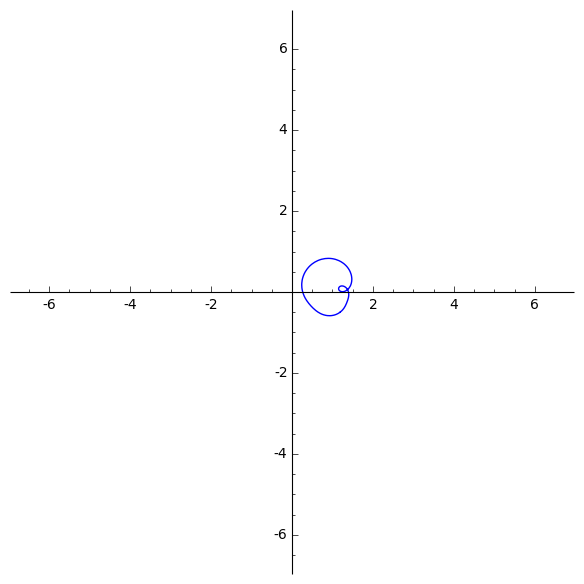
\includegraphics[scale=0.5]{figures/polynome1.png}\\$r_0 = 0.5$}
\only<2>{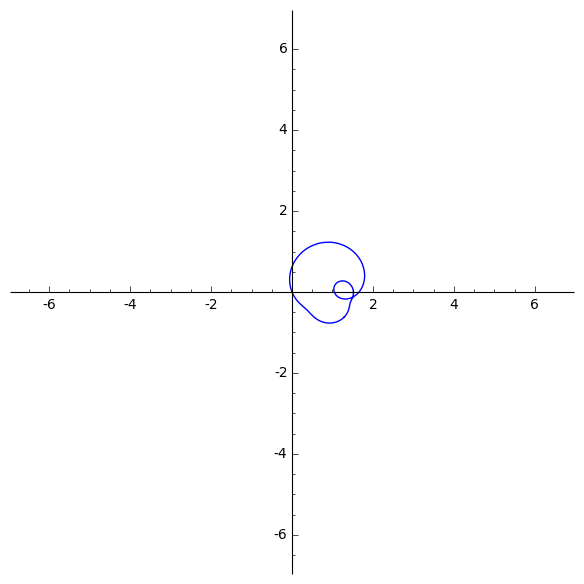
\includegraphics[scale=0.5]{figures/polynome2.png}\\$r_1 = 0.6176\ldots$}
\only<3>{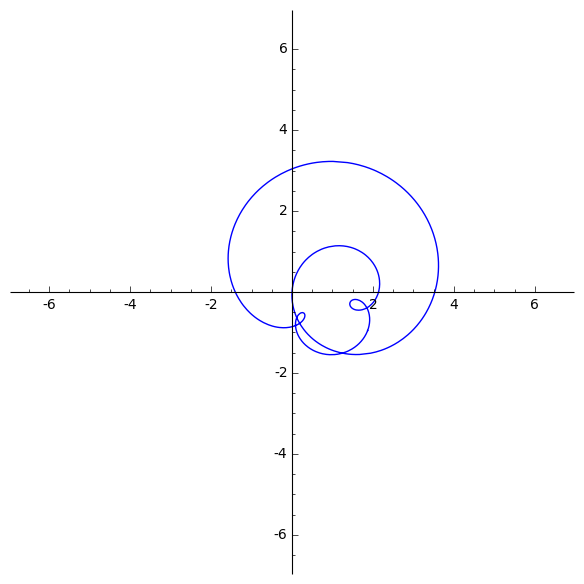
\includegraphics[scale=0.5]{figures/polynome3.png}\\$r_2 = 0.9534\ldots$}
\only<4>{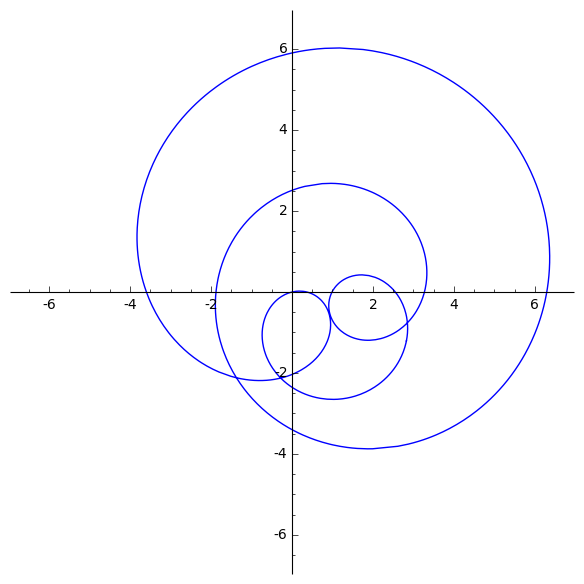
\includegraphics[scale=0.5]{figures/polynome4.png}\\$r_3 = 1.2082\ldots$}
\only<5>{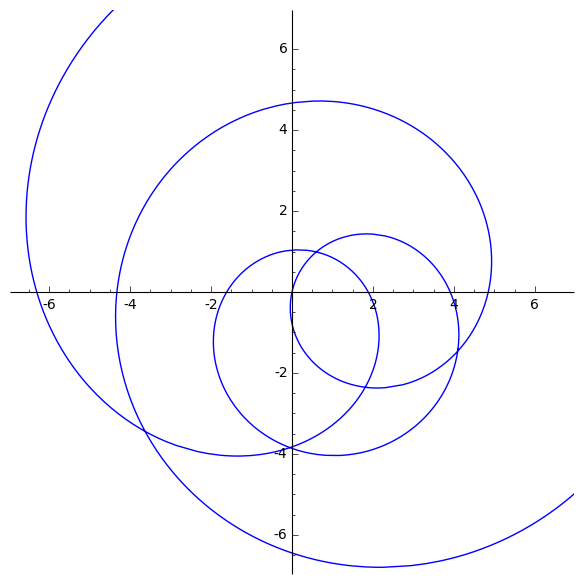
\includegraphics[scale=0.5]{figures/polynome5.png}\\$r_4 = 1.4055\ldots$}
\only<6>{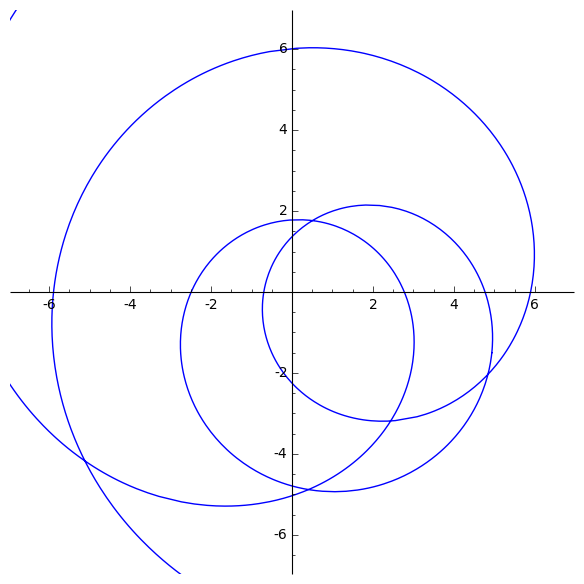
\includegraphics[scale=0.5]{figures/polynome6.png}\\$r_5 = 1.5$} 
\end{center}
\end{frame}


\begin{frame}[fragile]

\begin{algo}[intro-polynome.sage]
\begin{lstlisting}
R.<X> = CC[]
P = X^4-X^3+X^2-I*X+1|\pause|

def plot_image_cercle(P,r):
    var('t')
    zreal = P(r*exp(I*t)).real()
    zimag = P(r*exp(I*t)).imag()
    G = parametric_plot( (zreal,zimag), (t,0,2*pi) ) 
    return G|\pause|
    
A = animate( [plot_image_cercle(P,r) for r in srange(0.5,1.5,0.05)] )
A.show()

\end{lstlisting}
\end{algo}
\end{frame}

% for modz in [0.5,0.61...,0.95...,1.20...,1.40...,1.5]:
    % G = plot_image_cercle(P,modz)
    % G.show(xmin=-6, ymin=-6, xmax=6, ymax=6, axes=True) 


%%%%%%%%%%%%%%%%%%%%%%%%%%%%%%%%%%%%%%%%%%%%%%%%%%%%%%%%%%%%%%%%
\section{Algorithme de Horner}

\begin{frame}

\evidence{Algorithme de Horner} pour le calcul de $P(\alpha)$

\medskip
\pause

$P(X) = X^5 + X^4 - 5X^3 - 3X - 2$ \qquad $\alpha = 2$
\vspace*{-2ex}
\pause

\myfigure{0.8}{
\tikzinput{fig_formel_polynome01-diapo}
}

\pause\pause\pause\pause\pause
\pause\pause\pause\pause\pause
\pause\pause
\vspace*{-2ex}
$P(2)=0$

\pause
\medskip
\medskip

$P(X) = X^5 + X^4 - 5X^3 - 3X - 2$ \qquad $\alpha=-1$
\vspace*{-2ex}

\pause
\myfigure{0.8}{
\tikzinput{fig_formel_polynome02}
}

\pause
\vspace*{-2ex}
$P(-1)=6$
\end{frame}


\begin{frame}
\begin{tp}
On fixe un corps $K$ et un élément $\alpha$ de $K$. Soit $P(X) = a_nX^n+a_{n-1}X^{n-1}+\cdots +a_kX^k+\cdots+ a_1X+a_0 \in K[X]$.
%Fixons $\alpha \in K$. 

%Faire les applications avec 
%On pourra prendre pour les applications 
%$P(X) = X^5 + X^4 - 5X^3 - 3X - 2$ et $\alpha = 2$, puis $\alpha = -1$.


\begin{enumerate}
  \item Compter et comparer le nombre de multiplications nécessaires dans $K$ pour calculer 
  $P(\alpha)$, par :
 \begin{enumerate}
    \item le calcul direct :
    $$P(\alpha) = a_n \alpha^n+a_{n-1} \alpha^{n-1}+\cdots +a_k \alpha^k+\cdots+ a_1 \alpha +a_0,$$
    
    
    \item l'algorithme de Horner :
    $$P(\alpha) =  \Big(\big((a_n \alpha+a_{n-1})\alpha +a_{n-2} \big) \alpha + \cdots +a_1\Big) \alpha +a_0.$$
    \end{enumerate}

    \item \'Ecrire une fonction qui calcule $P(\alpha)$ par l'algorithme de Horner.
  \end{enumerate}
  \end{tp}
\end{frame}


\begin{frame}[fragile]
	\begin{enumerate}
  \item 
  \begin{enumerate}
    \item $P(\alpha) = a_n\alpha^n+a_{n-1}\alpha^{n-1}+\cdots +a_k\alpha^k+\cdots+a_1\alpha+a_0$
    
    \begin{itemize}
      \item monôme $a_k\cdot \alpha^ k$ :  $k$ multiplications
      \item $n+(n-1)+\cdots+k+\cdots+1+0 = \frac{n(n+1)}{2}$ multiplications (et $n$ additions)
    \end{itemize}
	
	 \pause
    
    \item $P(\alpha) =  \Big(\big((a_n \alpha+a_{n-1})\alpha +a_{n-2} \big) \alpha + \cdots + a_1\Big) \alpha +a_0$
    \begin{itemize}
      \item $n$ multiplications (et $n$ additions)
	
	 \pause      
      \item $b_{n} = a_n$ puis $b_{k} = \alpha b_{k+1}  + a_k$ pour $n-1\ge k \ge 0$
    \end{itemize}
     \pause
  \end{enumerate}    
    \item
\end{enumerate} 

%Pour l'implémentation, on note que la formule de récurrence 
 %   se fait pour des indices $k$ allant en décroissant.
  \begin{algo}[horner.sage]
\begin{lstlisting}
def eval_horner(P,alpha):
    n = P.degree()
    val = P[n]
    for k in range(n-1,-1,-1):
        val = alpha*val + P[k]
    return val
\end{lstlisting}
\end{algo}

\end{frame}
 



%%%%%%%%%%%%%%%%%%%%%%%%%%%%%%%%%%%%%%%%%%%%%%%%%%%%%%%%%%%%%%%%
\section{Interpolation de Lagrange}

\begin{frame}
\begin{theoreme}[Interpolation de Lagrange]
Soient $(x_i,y_i)$, $i=0,\ldots,n$, une suite de $n+1$ points, d'abscisses deux à deux distinctes. 
Il existe un unique polynôme $P$ de degré inférieur ou égal à $n$ tel que
$$P(x_i)=y_i \quad \text{ pour } i=0,\ldots,n.$$
\end{theoreme}

\pause
\bigskip

Application : 
pour une $f$ fonction continue sur un intervalle contenant $x_0,\ldots,x_n$, 
il existe un unique polynôme $P$ de degré inférieur à $n$ tel que
$$P(x_i)=f(x_i) \quad \text{ pour } i=0,\ldots,n.$$

\end{frame}


\begin{frame}
\begin{tp}
\begin{enumerate}
  \item Montrer l'unicité du polynôme $P$ dans le théorème d'interpolation de Lagrange. \pause 
  
  \item Pour l'existence, étant donnés $x_0,\ldots, x_n$, on définit les polynômes de Lagrange $L_0,L_1,\ldots,L_n$:
  $$L_i(X) = \prod_{j \neq i} \frac{X-x_j}{x_i-x_j}.$$
  Montrer que le polynôme :
  $P(X) = \sum_{i=0}^{n} y_i L_i(X)$
  répond au problème, c'est-à-dire que $P(x_i)=y_i$ ($i=0,\ldots,n$) et $\deg P \le n$.
  \pause
  \item \'Ecrire une fonction qui, étant donnée une liste de points, renvoie le polynôme
  d'interpolation $P$. Application à $f(x) = \sin(2\pi x)e^{-x}$
  sur l'intervalle $[0,2]$ avec une subdivision régulière de $n+1$ points.
  Tracer les graphes de la fonction $f$ et des polynômes d'interpolation
  correspondant à différentes valeurs de $n$.
  
  % \item Faire le même travail avec la fonction définie par $f(x) = \frac{1}{1+8x^2}$
  % sur l'intervalle $[-1,1]$, avec une subdivision régulière de $n+1$ points.
  % Quel problème apparaît ? C'est le \emph{phénomène de Runge}.
\end{enumerate}
\end{tp}
\end{frame}

 \begin{frame}
\begin{enumerate}
  \item Soient $P$ et $Q$ deux polynômes de degré inférieur à $n$ vérifiant
   $P(x_i)=Q(x_i)=y_i$
   \pause
   \begin{itemize}
     \item alors $P-Q$ vérifie $(P-Q)(x_i)=0$, $i=0,\ldots,n$ 
     \pause
     \item $\deg(P-Q)\leq n$ et $P-Q$ a $n+1$ racines distinctes 
     \pause
     \item ainsi $P-Q=0$, donc $P=Q$
   \end{itemize}
  
  \bigskip
  \pause
  \item $L_i(X) = \displaystyle \prod_{j \neq i} \frac{X-x_j}{x_i-x_j}$
  \pause
  \begin{itemize}
    \item $\deg(L_i)=n$ 
    \pause  
    \item $L_i(x_i) = 1$  et $L_i(x_j)=0$ pour $j\neq i$ 
    \pause  
    \item donc $P(X) = \sum_{j=0}^{n} y_j L_j(X)$ vérifie $\deg P \leq n$ 
    \pause
    \item et $P(x_i)= \sum_{j=0}^{n} y_j L_j(x_i) = y_iL_i(x_i) = y_i$ ($i=0,\ldots,n$)
  \end{itemize}  
  
  \bigskip   
  \pause 
   
  \item 
  \begin{itemize}
    \item \codeinline{R.<X> = RR[]}
    \pause   
    \item \codeinline{f = sin(2*pi*x)*exp(-x)}
    \pause
    \item \codeinline{liste_points =[(2*i/n,f(x=2*i/n)) for i in range(n+1)]} 
  \end{itemize}
  \end{enumerate}
 \end{frame}


\begin{frame}[fragile]
\begin{algo}[interpolation.sage]
\begin{lstlisting}
def interpolation_lagrange(liste_points):
    n = len(liste_points)-1
    allx = [p[0] for p in liste_points]
    ally = [p[1] for p in liste_points]|\pause|
    liste_lagrange = []    
    for i in range(n+1):
       A = prod(X-x for x in allx if x != allx[i])        
       B = prod(allx[i]-x for x in allx if x != allx[i])
       L = A/B
       liste_lagrange.append(L)|\pause|   
    lagrange = sum( liste_lagrange[i]*ally[i] for i in range(n+1) )
    return lagrange
\end{lstlisting}
\end{algo}

\end{frame}

\begin{frame}
\begin{center}
\only<1>{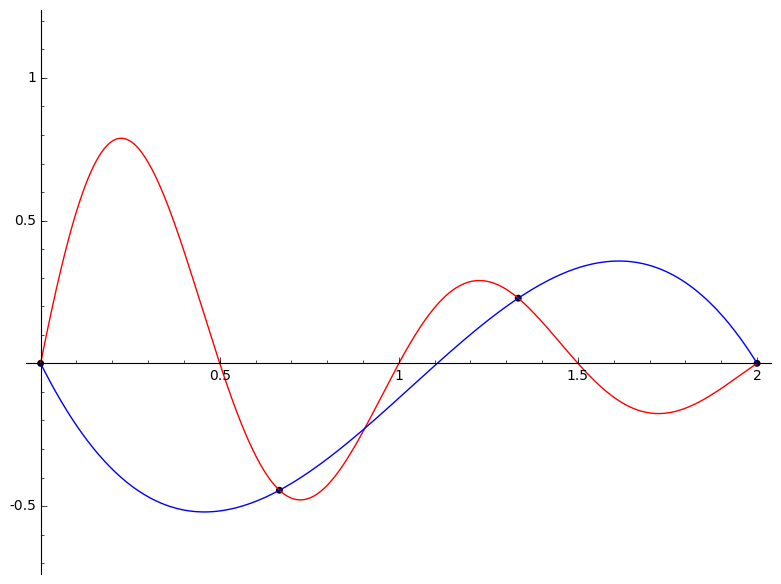
\includegraphics[scale=0.5]{figures/lagrange1.png}\\$n=3$}
\only<2>{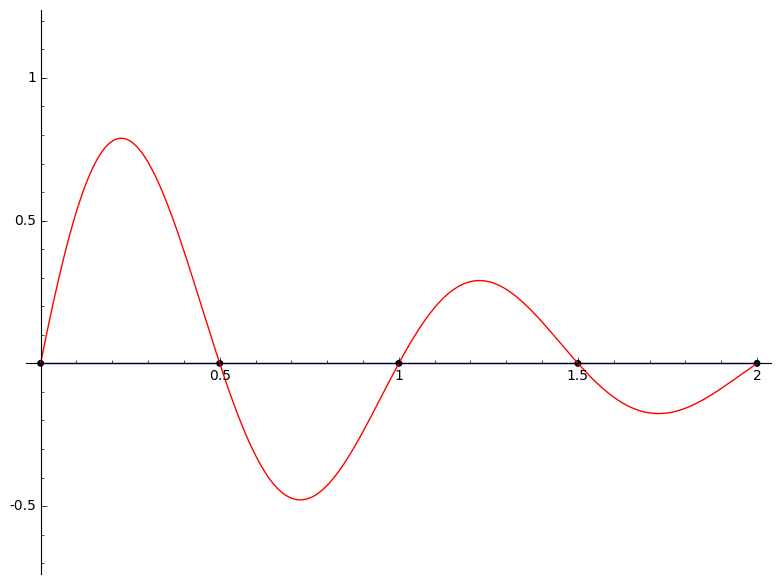
\includegraphics[scale=0.5]{figures/lagrange2.png}\\$n=4$}
\only<3>{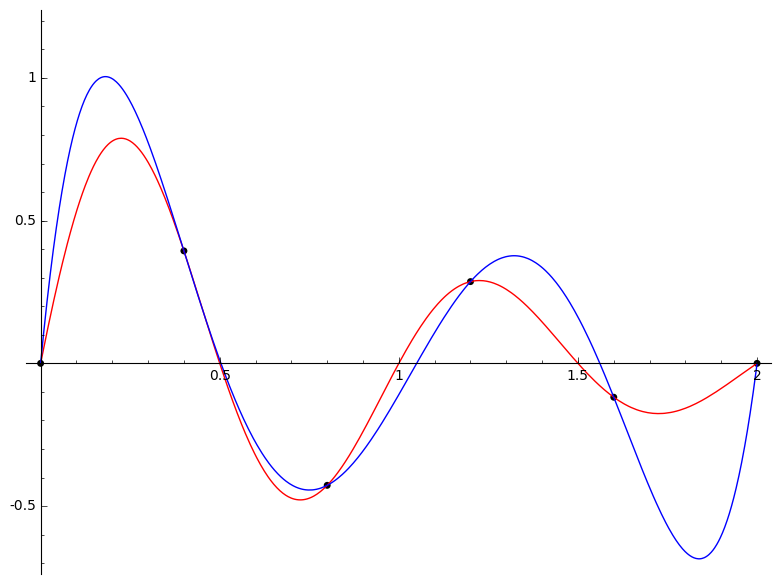
\includegraphics[scale=0.5]{figures/lagrange3.png}\\$n=5$}
\only<4>{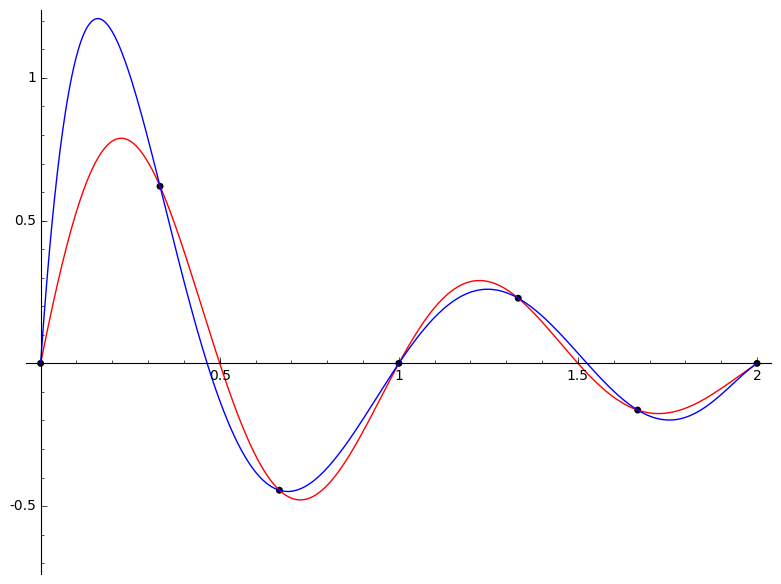
\includegraphics[scale=0.5]{figures/lagrange4.png}\\$n=6$}
\only<5>{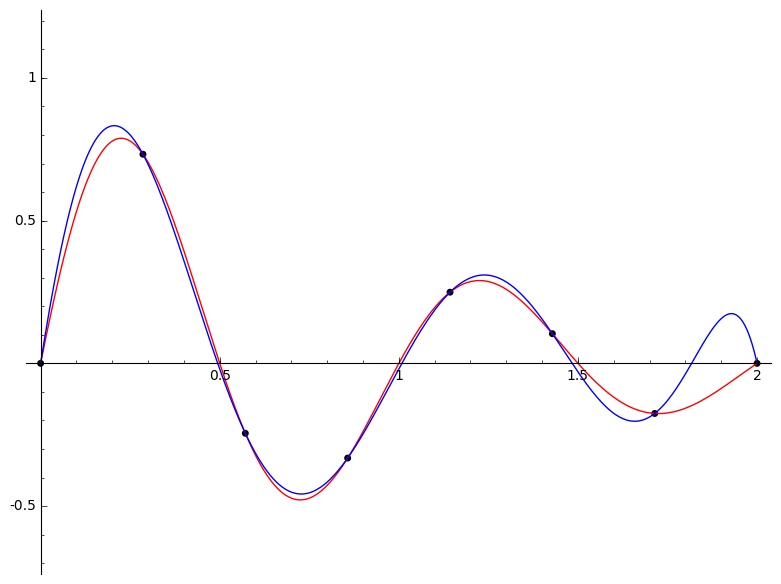
\includegraphics[scale=0.5]{figures/lagrange5.png}\\$n=7$}
\only<6>{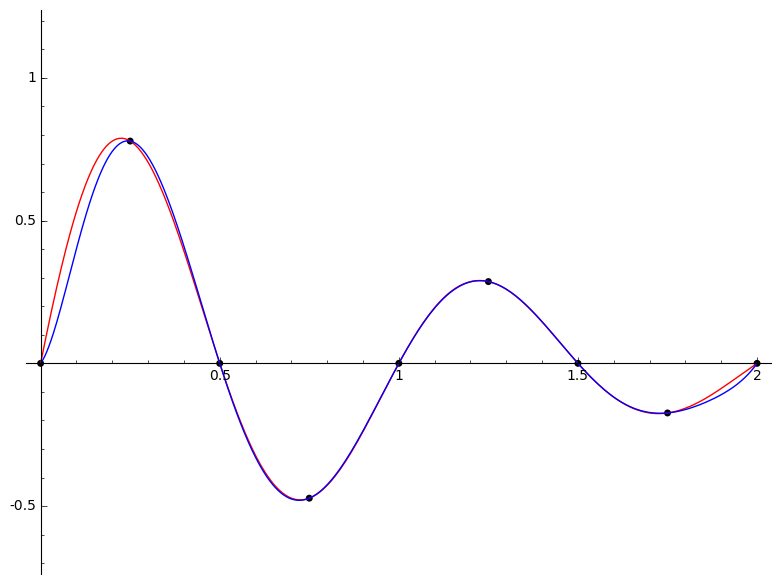
\includegraphics[scale=0.5]{figures/lagrange6.png}\\$n=8$}
\end{center}
\end{frame}


\end{document}
